%% toc: P2 11 11.7
\section{Post's five maximal classes and the functional-completeness criterion}
\label{sec:p02-w02-p02-008-post}
\index{functional completeness!Post's criterion}\index{clone!Boolean}

The definition of functional completeness in
Section~\ref{sec:prop-syntax-semantics-04} asks a set of connectives to
represent every truth function, and the basis theorem there exhibits one such
set, \(\{\neg,\land,\bottom\}\).  This section answers the general question:
which sets of connectives are functionally complete?  The answer is Post's
criterion.  A set is complete for truth functions of positive arity exactly
when, for each of five classes of truth functions, it contains a connective
whose truth function lies outside that class; the five classes are the
\(0\)-preserving, the \(1\)-preserving, the self-dual, the monotone and the
affine functions.  The criterion is stated and proved for clones, the sets of
truth functions closed under composition, and transferred to connective sets
by an exact correspondence between formulas and clones.

\emph{Inputs.}  The truth values, valuations and coincidence lemma
\cref{lem:prop-coincidence} of Section~\ref{sec:prop-syntax-semantics-02};
the truth-functional connectives, the formulas over a connective set, the
truth function of a formula in given variables, and the definition of
functional completeness, all from Section~\ref{sec:prop-syntax-semantics-04}.
\emph{Conclusions.}  Generated clones and their correspondence with formulas
(\cref{thm:p02-w02-p02-008-generated,thm:p02-w02-p02-008-formulas-clone});
the separation of positive-arity completeness from completeness that includes
nullary functions (\cref{thm:p02-w02-p02-008-nullary}); exact membership tests
for the five classes (\cref{thm:p02-w02-p02-008-tests},
Table~\ref{tab:p02-w02-p02-008-tests}); Post's criterion
(\cref{thm:p02-w02-p02-008-criterion}); the identification of the five classes
as exactly the maximal clones (\cref{thm:p02-w02-p02-008-maximal}); the
NAND and NOR constructions and the fact that these are the only binary truth
functions complete on their own
(\cref{thm:p02-w02-p02-008-nand-nor,thm:p02-w02-p02-008-sheffer}); negative
and positive basis examples (\cref{thm:p02-w02-p02-008-bases}); and the
upper part of the inclusion diagram of clones
(Figure~\ref{fig:p02-w02-p02-008-clones}).  Every proof is in the annex.

\subsection{Boolean operations, composition and clones}
\label{sec:p02-w02-p02-008-clones}

\begin{hbconvention}{def:p02-w02-p02-008-bits}{Truth values as bits}
In this section the truth values \(\mathbf F\) and \(\mathbf T\) are written
\(0\) and \(1\), and \(\mathbb B=\{0,1\}\).  For \(n\geq1\) a member of
\(\mathbb B^n\) is written \(\bar a=(a_1,\ldots,a_n)\); \(\bar0\) and
\(\bar1\) are the tuples with every coordinate \(0\), respectively \(1\);
\(\bar a\leq\bar b\) means \(a_i\leq b_i\) for every \(i\);
\(\bar a^{\,c}=(1-a_1,\ldots,1-a_n)\) is the complement of \(\bar a\); and
for \(1\leq i\leq n\) and \(b\in\mathbb B\), \(\bar a[i{:=}b]\) is the
tuple that agrees with \(\bar a\) except that its \(i\)-th coordinate is
\(b\).  On \(\mathbb B\), \(x\oplus y\) is addition modulo \(2\) and \(xy\)
is multiplication, so \(x\oplus y=1\) iff exactly one of \(x,y\) is \(1\),
\(1\oplus x=1-x\), and \(xy=1\) iff \(x=y=1\).  Iterated sums and products
are taken in any order and grouping, which is harmless because \(\oplus\)
and multiplication are associative and commutative and multiplication
distributes over \(\oplus\); the empty sum is \(0\) and the empty product is
\(1\).
\end{hbconvention}

\begin{hbdefinition}{def:p02-w02-p02-008-operations}{Boolean operation, composition, clone}
For \(n\geq1\), an \emph{\(n\)-ary Boolean operation} is a function
\(f:\mathbb B^n\to\mathbb B\); \(\mathcal O_n\) is the set of them and
\(\mathcal O=\bigcup_{n\geq1}\mathcal O_n\).  The \emph{arity} of
\(f\in\mathcal O_n\) is \(n\).  For \(1\leq i\leq n\), the \emph{projection}
\(e^n_i\in\mathcal O_n\) sends \(\bar a\) to \(a_i\); for
\(b\in\mathbb B\), the \emph{constant operation} \(\kappa^n_b\in\mathcal O_n\)
sends every \(\bar a\) to \(b\).  If \(f\in\mathcal O_m\) and
\(g_1,\ldots,g_m\in\mathcal O_n\), the \emph{composition}
\(f\circ(g_1,\ldots,g_m)\in\mathcal O_n\) sends \(\bar a\) to
\(f(g_1(\bar a),\ldots,g_m(\bar a))\).

A \emph{clone} is a set \(K\subseteq\mathcal O\) that contains every
projection \(e^n_i\) (\(n\geq1\), \(1\leq i\leq n\)) and is closed under
composition: whenever \(f\in K\cap\mathcal O_m\) and
\(g_1,\ldots,g_m\in K\cap\mathcal O_n\), also
\(f\circ(g_1,\ldots,g_m)\in K\).  For \(C\subseteq\mathcal O\), the
\emph{clone generated by \(C\)}, written \(\langle C\rangle\), is the
intersection of all clones \(K\) with \(C\subseteq K\); \(\mathcal O\) is
one of them, so the intersection is over a nonempty family.  A clone is
\emph{proper} iff it is not \(\mathcal O\), and \emph{maximal} iff it is
proper and the only clone properly including it is \(\mathcal O\).
\index{clone!generated}\index{clone!maximal}\index{Boolean operation}
\end{hbdefinition}

The connectives used below also name Boolean operations: \(\neg\) is the
unary operation \(x\mapsto1\oplus x\); \(\land,\lor,\to,\leftrightarrow\) and
\(\oplus\) are the binary operations with values \(xy\),
\(x\oplus y\oplus xy\), \(1\oplus x\oplus xy\), \(1\oplus x\oplus y\) and
\(x\oplus y\); \(\mathrm{NAND}(x,y)=1\oplus xy\) and
\(\mathrm{NOR}(x,y)=(1\oplus x)(1\oplus y)\); and the ternary
\emph{majority} operation \(\operatorname{maj}(x,y,z)\) is \(1\) iff at least
two of its arguments are \(1\).  For \(\neg,\land,\lor,\to\) these values
agree with the recursive truth clauses of
Section~\ref{sec:prop-syntax-semantics-02}; a connective symbol
\(\leftrightarrow\), \(\oplus\), \(\mathrm{NAND}\), \(\mathrm{NOR}\) or
\(\operatorname{maj}\) in a connective set is interpreted by the operation of
the same name.

\begin{hbconvention}{def:p02-w02-p02-008-arity}{Arity and constants}
Clones contain operations of positive arity only.  A set \(C\) of
truth-functional connectives in the sense of
Section~\ref{sec:prop-syntax-semantics-04} may contain nullary connectives
such as \(\bottom\).  Its \emph{operation set} \(C^+\subseteq\mathcal O\)
contains the interpreting operation of each member of positive arity and, for
each nullary member whose fixed value is \(b\), the unary constant operation
\(\kappa^1_b\).  So \(\bottom\) enters \(C^+\) as \(\kappa^1_0\) and a
nullary verum as \(\kappa^1_1\).  No clone contains a nullary function;
statements about nullary truth functions are made separately, through
\cref{thm:p02-w02-p02-008-nullary}.
\end{hbconvention}

\begin{hblemma}{thm:p02-w02-p02-008-generated}{proved=annex:p02-w02-p02-008-gen}{Generated clones}
Let \(C,D\subseteq\mathcal O\).
\begin{enumerate}
\item \(\langle C\rangle\) is a clone and \(C\subseteq\langle C\rangle\).
\item If \(K\) is a clone and \(C\subseteq K\), then
  \(\langle C\rangle\subseteq K\).
\item If \(C\subseteq\langle D\rangle\), then
  \(\langle C\rangle\subseteq\langle D\rangle\); in particular
  \(C\subseteq D\) implies \(\langle C\rangle\subseteq\langle D\rangle\).
\item If \(K\) is a clone, then \(\langle K\rangle=K\).
\item For a clone \(K\): \(\langle C\rangle\subseteq K\) iff
  \(C\subseteq K\).
\end{enumerate}
\end{hblemma}

\begin{hbdefinition}{def:p02-w02-p02-008-completeness}{Two scopes of functional completeness}
Let \(C\) be a set of truth-functional connectives.  For \(n\geq0\), a formula
over \(C\) \emph{represents} \(f:\mathbb B^n\to\mathbb B\) iff its variables
are among \(p_1,\ldots,p_n\) and its truth function in those variables is
\(f\).  \(C\) is \emph{positive-arity functionally complete} iff every
\(f:\mathbb B^n\to\mathbb B\) with \(n\geq1\) is represented by a formula
over \(C\).  \(C\) is \emph{nullary-inclusive functionally complete} iff the
same holds for every \(n\geq0\).  For \(n=0\), \(\mathbb B^0\) has exactly
one member, the empty tuple, so the two nullary truth functions are the two
constants, and a formula represents one of them only if it contains no
variable.  The definition of functional completeness in
Section~\ref{sec:prop-syntax-semantics-04} quantifies over every
\(n\in\N\), \(n=0\) included; it is the nullary-inclusive notion.
\index{functional completeness!positive arity}
\index{functional completeness!nullary inclusive}
\end{hbdefinition}

\begin{hbtheorem}{thm:p02-w02-p02-008-formulas-clone}{proved=annex:p02-w02-p02-008-formulas}{Formulas compute the generated clone}
Let \(C\) be a set of truth-functional connectives and \(n\geq1\).  An
operation \(f\in\mathcal O_n\) is represented by a formula over \(C\) iff
\(f\in\langle C^+\rangle\).  Consequently \(C\) is positive-arity
functionally complete iff \(\langle C^+\rangle=\mathcal O\).
\end{hbtheorem}

\begin{hbtheorem}{thm:p02-w02-p02-008-nullary}{proved=annex:p02-w02-p02-008-nullary}{Nullary functions need a nullary connective}
Let \(C\) be a set of truth-functional connectives.
\begin{enumerate}
\item If \(C\) has no nullary member, every formula over \(C\) contains a
  propositional variable; so neither nullary truth function is represented,
  and \(C\) is not nullary-inclusive functionally complete.
\item \(C\) is nullary-inclusive functionally complete iff \(C\) is
  positive-arity functionally complete and has at least one nullary member.
\end{enumerate}
\end{hbtheorem}

\subsection{The five classes and their membership tests}
\label{sec:p02-w02-p02-008-classes}

\begin{hbdefinition}{def:p02-w02-p02-008-five}{Post's five classes}
For \(f\in\mathcal O_n\), \(n\geq1\):
\begin{enumerate}
\item \(f\in\mathsf T_0\) (\(f\) \emph{preserves \(0\)}) iff
  \(f(\bar0)=0\);
\item \(f\in\mathsf T_1\) (\(f\) \emph{preserves \(1\)}) iff
  \(f(\bar1)=1\);
\item \(f\in\mathsf S\) (\(f\) is \emph{self-dual}) iff
  \(f(\bar a^{\,c})=1-f(\bar a)\) for every \(\bar a\in\mathbb B^n\);
\item \(f\in\mathsf M\) (\(f\) is \emph{monotone}) iff
  \(\bar a\leq\bar b\) implies \(f(\bar a)\leq f(\bar b)\);
\item \(f\in\mathsf L\) (\(f\) is \emph{affine}) iff there are
  \(c_0,c_1,\ldots,c_n\in\mathbb B\) with
  \(f(\bar a)=c_0\oplus c_1a_1\oplus\cdots\oplus c_na_n\) for every
  \(\bar a\in\mathbb B^n\).
\end{enumerate}
\index{self-dual truth function}\index{monotone truth function}
\index{affine truth function}
\end{hbdefinition}

\begin{hblemma}{thm:p02-w02-p02-008-tests}{proved=annex:p02-w02-p02-008-tests}{Exact membership tests}
Let \(f\in\mathcal O_n\), \(n\geq1\).
\begin{enumerate}
\item \(f\in\mathsf S\) iff \(f(\bar a^{\,c})\neq f(\bar a)\) for every
  \(\bar a\) with \(a_1=0\).
\item \(f\in\mathsf M\) iff \(f(\bar a)\leq f(\bar a[i{:=}1])\) for every
  \(\bar a\) and every \(i\) with \(a_i=0\).  Hence \(f\notin\mathsf M\) iff
  there are \(\bar a\) and \(i\) with \(a_i=0\), \(f(\bar a)=1\) and
  \(f(\bar a[i{:=}1])=0\).
\item Put \(c_0=f(\bar0)\) and \(c_i=f(\bar0[i{:=}1])\oplus f(\bar0)\) for
  \(1\leq i\leq n\).  Then \(f\in\mathsf L\) iff
  \(f(\bar a)=c_0\oplus c_1a_1\oplus\cdots\oplus c_na_n\) for every
  \(\bar a\).  If \(f\in\mathsf L\), these are the only coefficients that
  satisfy the condition of \cref{def:p02-w02-p02-008-five}.
\end{enumerate}
\end{hblemma}

With the defining conditions for \(\mathsf T_0\) and \(\mathsf T_1\), which
need one evaluation each, the lemma reduces every membership question to a
finite inspection of the truth table.
Table~\ref{tab:p02-w02-p02-008-tests} collects the five tests; the counts
assume the full truth table of an \(n\)-ary operation is given.

\begingroup\small
\begin{longtable}{@{}p{0.07\textwidth}p{0.25\textwidth}p{0.4\textwidth}p{0.18\textwidth}@{}}
\caption{The five maximal clones of Boolean operations and their exact
membership tests for \(f\in\mathcal O_n\), \(n\geq1\)
(\cref{def:p02-w02-p02-008-five,thm:p02-w02-p02-008-tests,thm:p02-w02-p02-008-maximal}).
Post's names for the same classes are in the last column
(Section~\ref{sec:p02-w02-p02-008-relationships}).}
\label{tab:p02-w02-p02-008-tests}\\
\toprule
Class & Defining condition & Exact test on the truth table & Post's system \\
\midrule\endfirsthead
\toprule
Class & Defining condition & Exact test on the truth table & Post's system \\
\midrule\endhead
\(\mathsf T_0\) & \(f(\bar0)=0\) & read the row \(\bar0\) (one entry) & \(C_3\) \\
\(\mathsf T_1\) & \(f(\bar1)=1\) & read the row \(\bar1\) (one entry) & \(C_2\) \\
\(\mathsf S\) & \(f(\bar a^{\,c})=1-f(\bar a)\) for all \(\bar a\)
 & \(f(\bar a^{\,c})\neq f(\bar a)\) for the \(2^{n-1}\) rows with
   \(a_1=0\) & \(D_3\) \\
\(\mathsf M\) & \(\bar a\leq\bar b\Rightarrow f(\bar a)\leq f(\bar b)\)
 & \(f(\bar a)\leq f(\bar a[i{:=}1])\) for the \(n2^{n-1}\) pairs with
   \(a_i=0\) & \(A_1\) \\
\(\mathsf L\) & \(f=c_0\oplus c_1a_1\oplus\cdots\oplus c_na_n\)
 & compute \(c_0=f(\bar0)\), \(c_i=f(\bar0[i{:=}1])\oplus c_0\), then
   check the identity on all \(2^n\) rows & \(L_1\) \\
\bottomrule
\end{longtable}
\endgroup

\begin{hblemma}{thm:p02-w02-p02-008-profile}{proved=annex:p02-w02-p02-008-profile}{Membership profile of the named operations}
For each operation in the first column of
Table~\ref{tab:p02-w02-p02-008-profile}, the classes among \(\mathsf T_0\), \(\mathsf T_1\),
\(\mathsf S\), \(\mathsf M\) and \(\mathsf L\) that contain it are
exactly those marked \(+\) in its row.
\end{hblemma}

\begingroup\small
\begin{longtable}{@{}lllccccc@{}}
\caption{Membership of named operations in the five classes; \(+\) marks
membership and \(-\) non-membership
(\cref{thm:p02-w02-p02-008-profile}).}
\label{tab:p02-w02-p02-008-profile}\\
\toprule
Operation & Arity & Values & \(\mathsf T_0\) & \(\mathsf T_1\) & \(\mathsf S\) & \(\mathsf M\) & \(\mathsf L\) \\
\midrule\endfirsthead
\toprule
Operation & Arity & Values & \(\mathsf T_0\) & \(\mathsf T_1\) & \(\mathsf S\) & \(\mathsf M\) & \(\mathsf L\) \\
\midrule\endhead
\(e^1_1\) & 1 & \(x\) & \(+\) & \(+\) & \(+\) & \(+\) & \(+\) \\
\(\neg\) & 1 & \(1\oplus x\) & \(-\) & \(-\) & \(+\) & \(-\) & \(+\) \\
\(\kappa^1_0\) & 1 & \(0\) & \(+\) & \(-\) & \(-\) & \(+\) & \(+\) \\
\(\kappa^1_1\) & 1 & \(1\) & \(-\) & \(+\) & \(-\) & \(+\) & \(+\) \\
\(\land\) & 2 & \(xy\) & \(+\) & \(+\) & \(-\) & \(+\) & \(-\) \\
\(\lor\) & 2 & \(x\oplus y\oplus xy\) & \(+\) & \(+\) & \(-\) & \(+\) & \(-\) \\
\(\to\) & 2 & \(1\oplus x\oplus xy\) & \(-\) & \(+\) & \(-\) & \(-\) & \(-\) \\
\(\leftrightarrow\) & 2 & \(1\oplus x\oplus y\) & \(-\) & \(+\) & \(-\) & \(-\) & \(+\) \\
\(\oplus\) & 2 & \(x\oplus y\) & \(+\) & \(-\) & \(-\) & \(-\) & \(+\) \\
\(\mathrm{NAND}\) & 2 & \(1\oplus xy\) & \(-\) & \(-\) & \(-\) & \(-\) & \(-\) \\
\(\mathrm{NOR}\) & 2 & \((1\oplus x)(1\oplus y)\) & \(-\) & \(-\) & \(-\) & \(-\) & \(-\) \\
\(\operatorname{maj}\) & 3 & at least two \(1\)s & \(+\) & \(+\) & \(+\) & \(+\) & \(-\) \\
\bottomrule
\end{longtable}
\endgroup

\begin{hblemma}{thm:p02-w02-p02-008-five-clones}{proved=annex:p02-w02-p02-008-five}{The five classes are proper clones}
Each of \(\mathsf T_0\), \(\mathsf T_1\), \(\mathsf S\), \(\mathsf M\)
and \(\mathsf L\) is a proper clone, and none of the five is included in another.
\end{hblemma}

\subsection{Post's criterion and the maximal clones}
\label{sec:p02-w02-p02-008-criterion}

Two auxiliary facts carry the sufficiency half of the criterion: negation and
conjunction already generate every operation, and every operation has an
algebraic normal form, a sum modulo \(2\) of products of distinct variables.

\begin{hblemma}{thm:p02-w02-p02-008-neg-and}{proved=annex:p02-w02-p02-008-neg-and}{Negation and conjunction generate every operation}
\(\langle\{\neg,\land\}\rangle=\mathcal O\).
\end{hblemma}

\begin{hblemma}{thm:p02-w02-p02-008-anf}{proved=annex:p02-w02-p02-008-anf}{Algebraic normal form}
For every \(n\geq1\) and \(f\in\mathcal O_n\) there is a set \(\mathcal J\)
of subsets of \(\{1,\ldots,n\}\) such that
\[
 f(\bar a)=\bigoplus_{J\in\mathcal J}\ \prod_{i\in J}a_i
 \qquad\text{for every }\bar a\in\mathbb B^n.
\]
If every member of some such \(\mathcal J\) has at most one element, then
\(f\in\mathsf L\).  Hence if \(f\notin\mathsf L\), every such \(\mathcal J\)
has a member with at least two elements.
\end{hblemma}

\begin{hbtheorem}{thm:p02-w02-p02-008-criterion}{proved=annex:p02-w02-p02-008-post}{Post's functional-completeness criterion}
\begin{enumerate}
\item For every \(C\subseteq\mathcal O\): \(\langle C\rangle=\mathcal O\)
  iff \(C\not\subseteq\mathsf T_0\), \(C\not\subseteq\mathsf T_1\),
  \(C\not\subseteq\mathsf S\), \(C\not\subseteq\mathsf M\) and
  \(C\not\subseteq\mathsf L\); that is, iff for each of the five classes
  some member of \(C\) lies outside it.
\item A set \(C\) of truth-functional connectives is positive-arity
  functionally complete iff its operation set \(C^+\) meets the condition of
  part~1.  It is nullary-inclusive functionally complete iff, in addition,
  \(C\) has a nullary member.
\end{enumerate}
\end{hbtheorem}

\begin{hbtheorem}{thm:p02-w02-p02-008-maximal}{proved=annex:p02-w02-p02-008-maximal}{The maximal clones}
\begin{enumerate}
\item Every proper clone is included in at least one of
  \(\mathsf T_0,\mathsf T_1,\mathsf S,\mathsf M,\mathsf L\).
\item Each of the five classes is a maximal clone.
\item A clone is maximal iff it is one of the five classes.  So
  \(\mathcal O\) has exactly five maximal subclones, and they are pairwise
  incomparable.
\end{enumerate}
\end{hbtheorem}

\begin{hbcorollary}{thm:p02-w02-p02-008-finite}{proved=annex:p02-w02-p02-008-finite}{A complete set has a complete subset of at most five members}
If \(C\subseteq\mathcal O\) and \(\langle C\rangle=\mathcal O\), then some
\(D\subseteq C\) with at most five members satisfies
\(\langle D\rangle=\mathcal O\).
\end{hbcorollary}

Post sharpens the bound for sets in which no member is generated by the
others: such a set, if it generates every operation, contains a function
whose diagonal is negation and at most two further members, or contains
functions whose diagonals are the two constants and at most two further
members; so it has at most four members, and Post lists all such sets in
fourteen forms \cite[\S\,26, pp.~105--107]{Post1941}.  That refinement is
reported here and not proved.

\begin{hbmethod}{def:p02-w02-p02-008-procedure}{Deciding functional completeness}
\emph{Input:} a finite set \(C\) of truth-functional connectives, each given
by its arity and truth table.  \emph{Output:} whether \(C\) is
positive-arity functionally complete, whether it is nullary-inclusive
functionally complete, and, when it is not complete for positive arities, a
class among the five that includes \(C^+\).
\begin{enumerate}
\item Form \(C^+\) by \cref{def:p02-w02-p02-008-arity}: replace each nullary
  member with value \(b\) by the unary operation \(\kappa^1_b\).
\item For each class \(K\) among \(\mathsf T_0,\mathsf T_1,\mathsf S,
  \mathsf M,\mathsf L\), apply the test of
  Table~\ref{tab:p02-w02-p02-008-tests} to the members of \(C^+\) until one
  fails it.  If every member passes the test for \(K\), stop: \(C^+\subseteq
  K\), and \(C\) is not positive-arity functionally complete.
\item If every class has a member of \(C^+\) outside it, \(C\) is
  positive-arity functionally complete.  It is nullary-inclusive
  functionally complete iff \(C\) also has a nullary member.
\end{enumerate}
\emph{Side conditions.}  The tests are exact by
\cref{thm:p02-w02-p02-008-tests}, and correctness of the verdicts is
\cref{thm:p02-w02-p02-008-criterion}.  Finiteness of \(C\) is needed only for
termination; the criterion itself holds for infinite sets.  The procedure
decides definability of all operations, not definability of one prescribed
operation; for the latter, see the containment argument of
\cref{thm:p02-w02-p02-008-bases}.  When the output is positive, the proof of
\cref{thm:p02-w02-p02-008-criterion} is constructive and yields explicit
compositions for negation, the two constants and conjunction, as in
\cref{def:p02-w02-p02-008-worked}.
\end{hbmethod}

\subsection{Single connectives: NAND and NOR}
\label{sec:p02-w02-p02-008-sheffer}
\index{Sheffer stroke}\index{NOR connective}

Basing a propositional calculus on a single primitive truth function goes back
to Sheffer and to Nicod, and Post names this as the stimulus for his
classification \cite[Introduction, p.~2]{Post1941}.  Here \(\mathrm{NAND}\)
and \(\mathrm{NOR}\) are binary connective symbols interpreted by the
operations \(\mathrm{NAND}(x,y)=1\oplus xy\) and
\(\mathrm{NOR}(x,y)=(1\oplus x)(1\oplus y)\) defined above; they are
connectives of the connective sets studied, not abbreviations within the
formula language of Section~\ref{sec:prop-syntax-semantics-01}.

\begin{hbtheorem}{thm:p02-w02-p02-008-nand-nor}{proved=annex:p02-w02-p02-008-nand-nor}{NAND and NOR}
\begin{enumerate}
\item In \(\mathcal O\), writing \(x\) for \(e^1_1\) and \(x,y\) for
  \(e^2_1,e^2_2\):
  \[
  \begin{aligned}
   \neg x&=\mathrm{NAND}(x,x),\\
   x\land y&=\mathrm{NAND}(\mathrm{NAND}(x,y),\mathrm{NAND}(x,y)),\\
   \kappa^1_1(x)&=\mathrm{NAND}(x,\mathrm{NAND}(x,x)),\\
   \kappa^1_0(x)&=\mathrm{NAND}(\kappa^1_1(x),\kappa^1_1(x)),
  \end{aligned}
  \]
  and
  \[
  \begin{aligned}
   \neg x&=\mathrm{NOR}(x,x),\\
   x\land y&=\mathrm{NOR}(\mathrm{NOR}(x,x),\mathrm{NOR}(y,y)),\\
   \kappa^1_0(x)&=\mathrm{NOR}(x,\mathrm{NOR}(x,x)),\\
   \kappa^1_1(x)&=\mathrm{NOR}(\kappa^1_0(x),\kappa^1_0(x)).
  \end{aligned}
  \]
\item \(\langle\{\mathrm{NAND}\}\rangle=\langle\{\mathrm{NOR}\}\rangle
  =\mathcal O\).  So each of the connective sets \(\{\mathrm{NAND}\}\) and
  \(\{\mathrm{NOR}\}\) is positive-arity functionally complete.
\item Neither \(\{\mathrm{NAND}\}\) nor \(\{\mathrm{NOR}\}\) is
  nullary-inclusive functionally complete; both
  \(\{\mathrm{NAND},\bottom\}\) and \(\{\mathrm{NOR},\bottom\}\) are.
\end{enumerate}
\end{hbtheorem}

\begin{hbcorollary}{thm:p02-w02-p02-008-sheffer}{proved=annex:p02-w02-p02-008-sheffer}{The singly complete operations of arity at most two}
No unary operation \(u\) satisfies \(\langle\{u\}\rangle=\mathcal O\).  A
binary operation \(f\) satisfies \(\langle\{f\}\rangle=\mathcal O\) iff
\(f\) is \(\mathrm{NAND}\) or \(\mathrm{NOR}\).
\end{hbcorollary}

So ``NAND alone is functionally complete'' is true for positive arities and
false in the nullary-inclusive sense of
Section~\ref{sec:prop-syntax-semantics-04}; the constants need a nullary
connective, by \cref{thm:p02-w02-p02-008-nullary}.

\subsection{Negative and positive bases}
\label{sec:p02-w02-p02-008-bases}

The criterion turns a non-definability claim into a containment check:
\(\langle C\rangle\subseteq K\) whenever \(C\subseteq K\) for a clone
\(K\), so no operation outside \(K\) is generated by \(C\), and by
\cref{thm:p02-w02-p02-008-formulas-clone} no formula over a connective set
\(C\) with \(C^+\subseteq K\) represents an operation outside \(K\).

\begin{hbtheorem}{thm:p02-w02-p02-008-bases}{proved=annex:p02-w02-p02-008-bases}{Negative and positive bases}
In each item, \(C\) is a set of operations; for a connective set, read
\(\bottom\) as \(\kappa^1_0\) and a nullary verum \(\topv\) as
\(\kappa^1_1\).  The classes listed are exactly those among the five that
include \(C\), and therefore exactly those that include
\(\langle C\rangle\).
\begin{enumerate}
\item \(\{\land,\lor\}\): \(\mathsf T_0,\mathsf T_1,\mathsf M\).  Neither
  \(\neg\) nor either constant operation lies in \(\langle C\rangle\).
\item \(\{\land,\lor,\kappa^1_0,\kappa^1_1\}\): \(\mathsf M\) only.  So the
  connective set \(\{\land,\lor,\bottom,\topv\}\) does not define negation.
\item \(\{\neg,\leftrightarrow\}\) and \(\{\neg,\oplus\}\): \(\mathsf L\)
  only, and the two generated clones are equal.  So neither set defines
  \(\land\), \(\lor\) or \(\to\).
\item \(\{\to\}\): \(\mathsf T_1\) only.  So implication alone defines
  neither \(\neg\) nor \(\kappa^1_0\).
\item \(\{\land,\oplus\}\): \(\mathsf T_0\) only.  So it defines neither
  \(\neg\), \(\to\), \(\leftrightarrow\) nor \(\kappa^1_1\).
\item \(\{\neg,\operatorname{maj}\}\): \(\mathsf S\) only.  So it defines
  neither \(\land\), \(\lor\) nor either constant operation.
\item \(\{\to,\kappa^1_0\}\) and \(\{\land,\oplus,\kappa^1_1\}\): none.
  So the connective sets \(\{\to,\bottom\}\) and \(\{\land,\oplus,\topv\}\)
  are positive-arity and nullary-inclusive functionally complete.
\end{enumerate}
\end{hbtheorem}

\begin{figure}[tp]
\centering
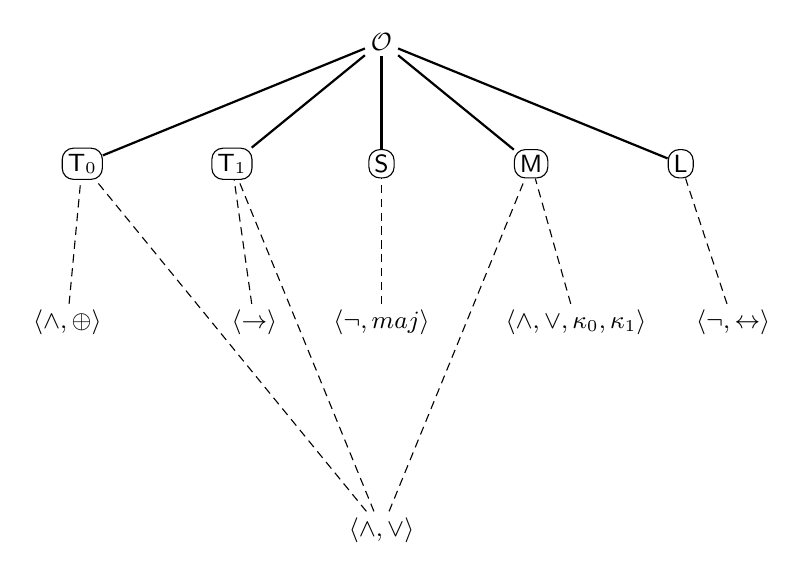
\begin{tikzpicture}[x=1.9cm,y=1.55cm,every node/.style={inner sep=2pt,font=\small}]
 \node (O) at (2,3) {\(\mathcal O\)};
 \node[draw,rounded corners] (t0) at (0,2) {\(\mathsf T_0\)};
 \node[draw,rounded corners] (t1) at (1,2) {\(\mathsf T_1\)};
 \node[draw,rounded corners] (s)  at (2,2) {\(\mathsf S\)};
 \node[draw,rounded corners] (m)  at (3,2) {\(\mathsf M\)};
 \node[draw,rounded corners] (l)  at (4,2) {\(\mathsf L\)};
 \foreach \k in {t0,t1,s,m,l} \draw[thick] (O)--(\k);
 \node (xa) at (-0.1,0.7) {\(\langle\land,\oplus\rangle\)};
 \node (im) at (1.15,0.7) {\(\langle\to\rangle\)};
 \node (nm) at (2,0.7) {\(\langle\neg,\operatorname{maj}\rangle\)};
 \node (mk) at (3.3,0.7) {\(\langle\land,\lor,\kappa_0,\kappa_1\rangle\)};
 \node (ne) at (4.35,0.7) {\(\langle\neg,\leftrightarrow\rangle\)};
 \node (aj) at (2,-1.0) {\(\langle\land,\lor\rangle\)};
 \draw[densely dashed] (xa)--(t0); \draw[densely dashed] (im)--(t1);
 \draw[densely dashed] (nm)--(s);  \draw[densely dashed] (mk)--(m);
 \draw[densely dashed] (ne)--(l);
 \draw[densely dashed] (aj)--(t0); \draw[densely dashed] (aj)--(t1);
 \draw[densely dashed] (aj)--(m);
\end{tikzpicture}
\caption{The top of the lattice of clones of Boolean operations.  Solid
lines: \(\mathcal O\) covers exactly the five boxed maximal clones
(\cref{thm:p02-w02-p02-008-maximal}).  Dashed lines: each lower node, the
clone generated by a basis of \cref{thm:p02-w02-p02-008-bases} (with
\(\kappa_b\) for \(\kappa^1_b\)), is joined to every maximal clone that
includes it, and to no other.  These are inclusions, not necessarily covers;
inclusions among the lower nodes and all other clones of the lattice, which
has infinitely many members, are not drawn.}
\label{fig:p02-w02-p02-008-clones}
\end{figure}

\begin{hbexample}{def:p02-w02-p02-008-worked}{Conjunction from implication and falsum}
Take the connective set \(\{\to,\bottom\}\), so \(C^+=\{\to,\kappa^1_0\}\).
By Table~\ref{tab:p02-w02-p02-008-profile}, \(\to\) lies outside
\(\mathsf T_0\), \(\mathsf S\), \(\mathsf M\) and \(\mathsf L\), and
\(\kappa^1_0\) lies outside \(\mathsf T_1\); the set is complete.  The proof
of \cref{thm:p02-w02-p02-008-criterion} then produces the following
formulas, each checked on its truth table.
\begin{enumerate}
\item \emph{Constants.}  The diagonal of \(\to\) is
  \(x\mapsto(x\to x)\), the constant \(1\), represented by
  \(p_1\to p_1\); the constant \(0\) is represented by \(\bottom\).
\item \emph{Negation.}  The monotonicity test fails for \(\to\) at
  \(\bar a=(0,0)\) and \(i=1\): \((0\to0)=1\) and \((1\to0)=0\).  Fixing
  the second argument at \(0\) gives \(\neg x=x\to0\), represented by
  \(p_1\to\bottom\).
\item \emph{Conjunction.}  The algebraic normal form of \(\to\) is
  \(1\oplus x\oplus xy\), with the single nonlinear monomial \(xy\).  In the
  notation of the proof, \(p(x,y)=xy\oplus x\oplus1\), so the coefficients
  are \(\alpha=1\), \(\beta=0\), \(\gamma=1\), and
  \(xy=p(x,\,1\oplus y)\oplus1\).  That is,
  \(x\land y=\neg(x\to\neg y)\), represented by
  \((p_1\to(p_2\to\bottom))\to\bottom\).  Its truth table is \(1\) only at
  \((1,1)\): there \(p_2\to\bottom\) is \(0\), \(p_1\to0\) is \(0\), and the
  outer implication gives \(1\); at every other row \(p_1\to(p_2\to\bottom)\)
  is \(1\) and the outer implication gives \(0\).
\end{enumerate}
From negation and conjunction, \cref{thm:p02-w02-p02-008-neg-and} supplies
every operation of positive arity, and the closed formulas \(\bottom\) and
\(\bottom\to\bottom\) supply the two nullary constants.
\end{hbexample}

\begin{hbwarning}{def:p02-w02-p02-008-limits}{Scope of the criterion}
\begin{enumerate}
\item The criterion is about expressibility: which truth functions are
  compositions of given ones.  It says nothing about derivability, and a
  complete connective set does not come with a complete calculus.
\item It is a positive-arity result.  Clones contain no nullary function,
  and a connective set without a nullary member is never nullary-inclusive
  functionally complete (\cref{thm:p02-w02-p02-008-nullary}); nullary
  constants of a language enter the criterion only as unary constant
  operations.
\item It is specific to two truth values.  The proof uses that there are
  exactly four unary operations on \(\mathbb B\) and that a
  non-monotone or non-affine operation over \(\mathbb B\) yields negation or
  conjunction; nothing here classifies operations on a set with more than
  two elements.
\item The criterion decides whether every operation is definable; it gives
  no bound on the size of the defining formulas.
\end{enumerate}
\end{hbwarning}

\subsection{Relationships and sources}
\label{sec:p02-w02-p02-008-relationships}

\emph{The basis theorem.}  The functionally complete basis
\(\{\neg,\land,\bottom\}\) of Section~\ref{sec:prop-syntax-semantics-04} is an
instance of \cref{thm:p02-w02-p02-008-criterion}: \(\neg\) lies outside
\(\mathsf T_0\) and \(\mathsf M\), \(\land\) outside \(\mathsf S\) and
\(\mathsf L\), and \(\kappa^1_0\) outside \(\mathsf T_1\); and \(\bottom\) is
a nullary member, so completeness is nullary-inclusive.

\emph{Post's classification.}  Post works with two-valued functions of
variables drawn from a fixed denumerable list, and calls a system of such
functions iteratively closed, or closed, when replacing the arguments of any
of its functions by variables or by functions of the system again gives a
function of the system \cite[\S\,1, pp.~10--11]{Post1941}.  He excludes
functions of no variables, that is, constants, from the classification
\cite[Introduction, pp.~2--3, n.~5]{Post1941}; this is the positive-arity
convention of \cref{def:p02-w02-p02-008-arity}.  In his notation the
complete system is \(C_1\); every closed system properly included in \(C_1\)
is included in at least one of \(C_2\), \(C_3\), \(D_3\), \(A_1\) and
\(L_1\), and none of these five is properly included in another
\cite[\S\,25, pp.~98--99]{Post1941}.  He concludes that a set of generators
yields the complete system exactly when each of the five fails to contain it
\cite[\S\,26, p.~105]{Post1941}.  The five systems are the five classes of
\cref{def:p02-w02-p02-008-five}, as follows.
\begin{itemize}
\item Post describes \(D_3\) as the system of all self-dual functions and
  \(L_1\) as the system of all alternating functions
  \cite[\S\,26, p.~106]{Post1941}.  So \(D_3=\mathsf S\).  A function is
  alternating when replacing any one argument by its negation either leaves
  the function unchanged or turns it into its negation
  \cite[\S\,15, p.~55]{Post1941}, and by
  \cref{thm:p02-w02-p02-008-alternating} below these are exactly the affine
  functions; so \(L_1=\mathsf L\).
\item Post sorts functions by the one-variable function obtained by
  identifying all arguments, calling a function an \(\alpha\)-,
  \(\beta\)-, \(\gamma\)- or \(\delta\)-function according as that function
  is the identity, the constant \(1\), the constant \(0\) or negation
  \cite[\S\,10, p.~43]{Post1941}.  He notes that a set of generators escapes
  \(C_2\) only if it has a \(\gamma\)- or \(\delta\)-function, and escapes
  \(C_3\) only if it has a \(\beta\)- or \(\delta\)-function
  \cite[\S\,26, p.~105]{Post1941}.  The \(\alpha\)- and
  \(\beta\)-functions are exactly the members of \(\mathsf T_1\), so
  \(\mathsf T_1\subseteq C_2\); since \(C_2\) is not the complete system and
  \(\mathsf T_1\) is maximal (\cref{thm:p02-w02-p02-008-maximal}),
  \(C_2=\mathsf T_1\).  In the same way the \(\alpha\)- and
  \(\gamma\)-functions are the members of \(\mathsf T_0\), and
  \(C_3=\mathsf T_0\).
\item Post's \(A_1\) is the system of all functions satisfying his
  \([A{:}a]\) condition \cite[\S\,26, p.~106]{Post1941}.  The clone
  \(\mathsf M\) is closed in Post's sense and is not \(\mathcal O\), so by
  his inclusion result it lies in one of the five systems; it lies in none of
  \(C_2=\mathsf T_1\), \(C_3=\mathsf T_0\), \(D_3=\mathsf S\),
  \(L_1=\mathsf L\), because \(\kappa^1_0\), \(\kappa^1_1\) and \(\land\)
  are monotone and lie outside \(\mathsf T_1\) and \(\mathsf S\),
  \(\mathsf T_0\), and \(\mathsf L\) respectively
  (Table~\ref{tab:p02-w02-p02-008-profile}).  So
  \(\mathsf M\subseteq A_1\), and maximality of \(\mathsf M\) gives
  \(A_1=\mathsf M\).  Consistently, Post records that every
  \(\delta\)-function fails the \([A{:}a]\) condition
  \cite[\S\,26, p.~106]{Post1941}, while a monotone \(f\) has
  \(f(\bar0)\leq f(\bar1)\) and so cannot have negation as its diagonal.
\end{itemize}
The proofs in the annex do not use this comparison; it fixes which of Post's
systems each table row names.

\begin{hblemma}{thm:p02-w02-p02-008-alternating}{proved=annex:p02-w02-p02-008-alt}{Alternating means affine}
For \(f\in\mathcal O_n\), \(f\in\mathsf L\) iff for every \(i\leq n\) either
\(f(\bar a[i{:=}1-a_i])=f(\bar a)\) for every \(\bar a\), or
\(f(\bar a[i{:=}1-a_i])=1-f(\bar a)\) for every \(\bar a\).
\end{hblemma}

\emph{The clone lattice.}  Post's classification is of all closed systems,
not only the maximal ones.  The set of closed systems is infinite
\cite[\S\,25, p.~96]{Post1941}, and Post draws the whole inclusion relation in
an inclusion diagram in which a downward line joins each system to each
system it immediately includes \cite[\S\,25, p.~100]{Post1941}.
Figure~\ref{fig:p02-w02-p02-008-clones} is the top of that two-valued
diagram: its five boxed nodes are Post's \(C_3\), \(C_2\), \(D_3\), \(A_1\)
and \(L_1\), and the lines from \(\mathcal O\) are the five immediate
inclusions under \(C_1\).  The classification concerns operations on the
two-element set \(\mathbb B\) only; nothing in this section concerns
truth functions with more than two values.

\emph{Elsewhere in this part.}  The normal forms of
Section~\ref{sec:prop-syntax-semantics-04} supply, in formula form, the
disjunctive construction behind \cref{thm:p02-w02-p02-008-neg-and}.
\index{Post's criterion}
